\documentclass[10pt]{report}
\usepackage{epsf}
\usepackage{amsmath}
\usepackage{amssymb}
\usepackage{float}
\usepackage{palatino}
\usepackage[pdftex]{graphics}
\usepackage{fancyhdr}
\usepackage[pdftex]{graphicx}
\usepackage{hyperref}
\parindent 0in
\parskip 1ex
\oddsidemargin  0in
\evensidemargin 0in
\textheight 8.5in
\textwidth 6.5in
\topmargin -0.25in

\pagestyle{fancy}
\fancyhf{}
\fancyhead[L]{\bf BME354L - Palmeri - Spring 2013}
\fancyhead[R]{{\bf Arduino Project}}
%\fancyfoot[L]{LICENSE: CC BC-NC-SA 3.0 ({\tt http://creativecommons.org/licenses/by-nc-sa/3.0/})}
\fancyfoot[C]{\thepage}

\title{What is a reflow oven?}
\author{Will Scheideler}
\begin{document}

\section*{What is a reflow oven?}

\subsection*{Introduction}

\par A reflow oven is an essential piece of equipment for electrical engineers that facilitates the soldering of electrical components. Reflow ovens are used on an industrial scale as part of a highly efficient and scalable process for bonding components to printed circuit boards. In Lab 5, you got some experience soldering the PICAXE demo board with several components on it. This experience gave you some idea of the low efficiency of soldering by hand. Reflow ovens allow you to solder components en masse.  They are used by developers (and students too!) to create complex circuits that can include surface mount components.

\par \indent \emph{Surface mount components} are a class of miniaturized electrical components that are bonded to the board with a thick metal solder paste. The small size of surface mount components makes them standard choices for use in many devices. You will find that many of the components which you have become familiar with in the laboratory (resistors, capacitors, microcontrollers, amplifiers, etc) have surface mount versions which are miniaturized for mounting on a printed circuit board. By including surface mount components rather than the through hole (the black epoxy packages you are used to seeing) components, manufacturing costs and device sizes are drastically reduced. For something like an implantable device, the miniaturization that surface mount components facilitate is essential.

\par \indent The Reflow process is performed by the reflow oven. Components are glued to the circuit board using solder paste and the ensemble is baked at a specified set of temperatures. The temperature profile for this process is shown below in Figure 1. The overarching goal of the process is to bring the temperature of the solder (and the component) above the solder melting temperature. The solder alloy is specifically designed to melt at a relatively low temperature (218 $^\circ$C) so that thermal stress on the electrical components may be minimized. Electrical devices are composed of semiconductors whose properties can change drastically with heat treatment annealing. Likewise, the quality of the solder joint is very dependent on achieving the specified temperature profile. This means that a reflow oven must achieve precise temperature control, within minimal deviations from the specified curve.  

\begin{figure}[H]
\centering
   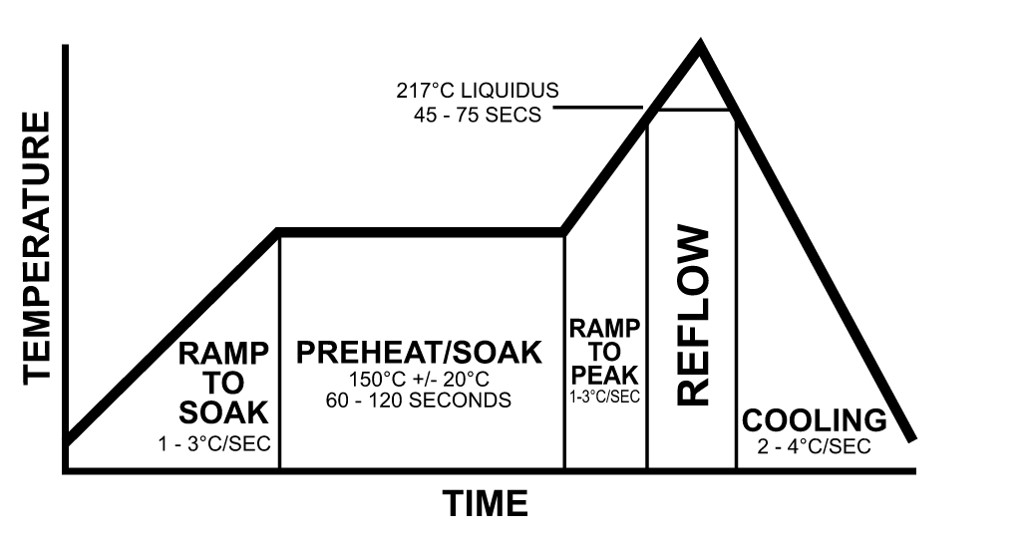
\includegraphics[width=0.7\textwidth]{reflow_Curve.jpg}
    \caption{A standard reflow temperature profile}
\end{figure}

\subsection*{The Reflow Process}
\par The reflow process may be broken down into several subsections described below:

\begin{itemize}
\item \textbf{Preheat} The temperature is increased from room temperature to 150 $^\circ$C. The ramp up rate must be 1-3 $^\circ$C/s. The upper bound for the ramp rate is 3 $^\circ$C/s due to risk of thermal shock for the components.

\item \textbf{Soak} The soak stage serves to remove oxides from the solder paste and activates the flux compounds. Soaking at too low a temperature may cause a solder ball to form.

\item \textbf{Reflow} At this stage, the solder paste reaches its melting point at the ‘liquidous’ temperature which is approximately 218 $^\circ$C for lead free solder paste (Sn-Ag-Cu based). The board must not remain above the liquidous temperature for more than the recommended 60-90 s. Once the peak reflow temperature is achieved, cooling begins.

\item \textbf{Cool} The cooling stage must have  ramp down rate of less than -6 $^\circ$C per second during the initial ramp down (245 - 200 $^\circ$C).

\end{itemize}

\par Achieving these steps in the specified order is essential to producing consistent solder joints. Without precise timing and temperature accuracy, the solder joints may not form, or they may form with unfavorable properties (high resistance). For analog circuits used in sensing (especially for Biomedical Engineering), the difference between a 0.2  solder joint and a 2  solder joint could potentially be quite important. 

\par The goal of the final design project will be to design a reflow oven. Here are the basic requirements of the oven you will design:


\begin{itemize}
\item Design a \emph{Control System}  that will control the temperature of a reflow oven by switching the ON/OFF state of a heating element.
	\begin{itemize}
	\item Constantly monitor temperatures to achieve the desired temperature profile.
	\item Include software based fail-safes...What temperatures are unsafe?
	\end{itemize}
\item Provide the capability to read \emph{User Input}.
	\begin{itemize}
	\item The user should enter the exact reflow curve (A finite set of temperatures and times) that their solder composition requires.
	\end{itemize}
\item 	Provide \emph{User Output}
	\begin{itemize}
	\item What is the current oven temperature?
	\item What stage of the reflow process is the oven current in?
	\item How much time is left in the current reflow run?
	\end{itemize}
\item Produce Statistics on the agreement of the actual reflow curve with the desired reflow curve.
	\begin{itemize}
	\item What was the desired peak temperature?
	\item What was the actual peak temperature?
	\item Quantify the error of the actual reflow curve?
	\end{itemize}
\item \emph{Autonomous Operation}
	\begin{itemize}
	\item After accepting user inputs, the oven should do its job without user intervention.
	\end{itemize}
\item \emph{Safety Considerations}
	\begin{itemize}
	\item You are working with a high current, high temperature device. Just like any other electrical device, and especially the case with medical devices, 		you will have to consider what safety measures need to be implemented. If the device fails, how do you ensure that the user (and internal 				components) are not harmed? What features in hardware and software might aid you in doing this? 

	\item What temperatures are safe? What range of temperatures should the user be allowed to specify?

	\item What fault conditions can you detect during a reflow run? What is an appropriate response to detecting such a condition. Can you give useful feedback to the user to let them know what went wrong? 
	\end{itemize}
\end{itemize}

\subsubsection{Extra Credit Extensions:}

\begin{itemize}
\item User Output
	\begin{itemize}
	\item Can you output the information on temperature, user chosen set points, etc. in a more usable form?
	\item Can you print information to the Arduino Serial Monitor?
	\item Can you print information to MATLAB / graph that information?
	\end{itemize}
\item User Interface
	\begin{itemize}
	\item What feedback is useful to the user?
	\item LED indicators? Buzzer indicators, etc?
	\end{itemize}
\item Sensing
	\begin{itemize}
	\item What is the resolution of your temperature measurement? What is it limited by?
	\item Could you improve the resolution with signal processing techniques? 
	\end{itemize}
\end{itemize}

\end{document}